\section{Experimentation \& Results}\label{results}

A number of computational experiments are conducted to highlight unique features
enabled by the DRE in Cyclus. Each experiment is performed by solving instances
of the DRE using both the greedy heuristic and to optimality with COINOR-CBC. A
UOX-MOX binary recycle system with all required fuel cycle facilities is taken
as a base-case scenario in order to reduce the complexity of the fuel cycle and
highlight departures from available simulators. A simulation timeframe of 50
years is chosen (totaling 600 simulation time steps), sufficient to display all
relevant effects. The nominal parameters of all common facilities in the
simulation are shown in Appendix \ref{}. Importantly, reactors are allowed to be
fueled by either UOX or MOX, with a preference for MOX over UOX. Spent UOX fuel
is allowed to be recycled, whereas spent MOX fuel is sent directly to a
repository. In order to involve dynamicism in the simulation, the population
reactors grows linearly over time at a rate of 1 reactor every 5 years. An
initial population of 20 reactors are deployed individually in each of the first
20 timesteps of the simulation. The diagram of the base-case fuel cycle is shown
in Figure \ref{fig:base}.

\begin{figure}
  \begin{center}
    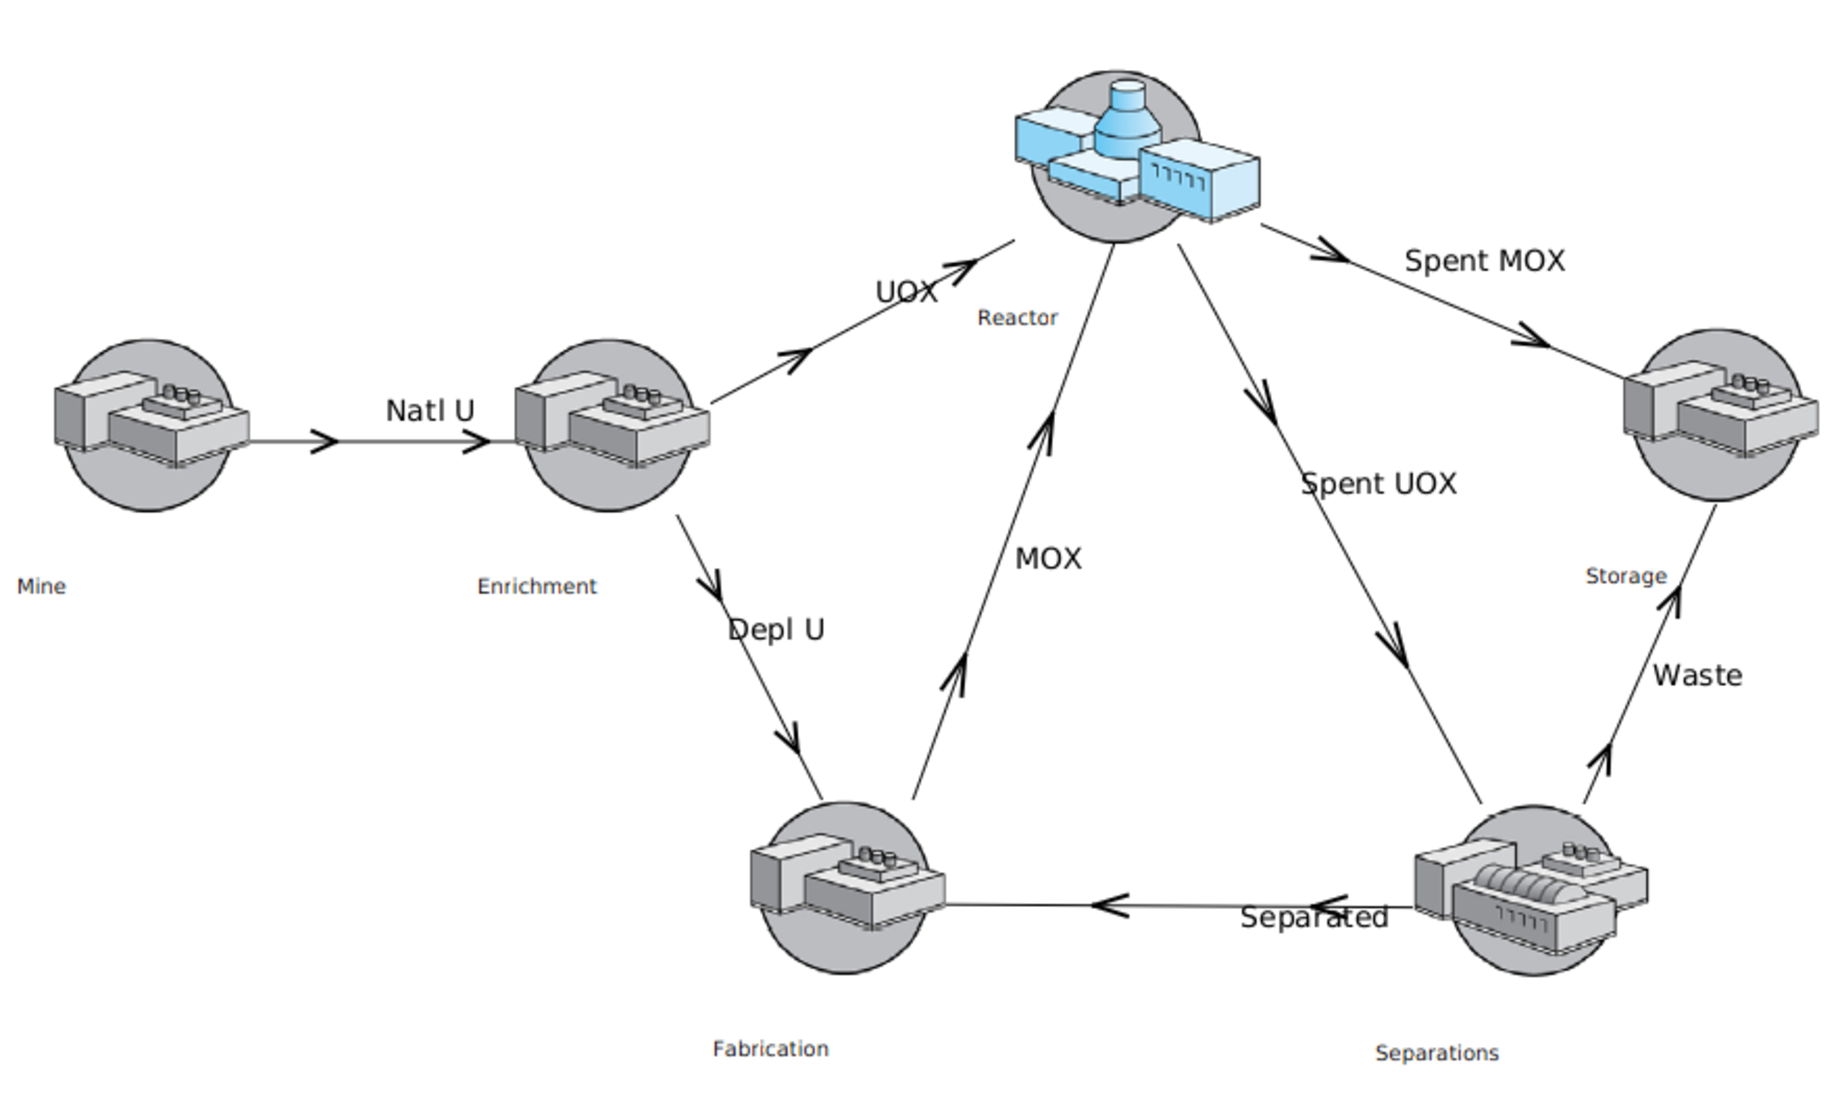
\includegraphics[width=\columnwidth]{base.pdf}
    \caption[]{
      \label{fig:base}
      Material routing between in the base-case, single-pass MOX fuel
      cycle. Possible arc flows are labeled with commodity names.}
  \end{center}
\end{figure}

\subsection{Description of Scenarios}

Four perturbations from the base-case scenario are used to provide examples of
modeling capability enabled through the use of the DRE. The scenarios are
summarized in Table \ref{scenarios} below and described in more detail in the
following sections.

\begin{table}[]
\centering
\caption{Short Descriptions of Scenarios Ran}
\label{scenarios}
\begin{tabularx}{\textwidth}{|p{1.5cm}|p{1.5cm}|X|X|}
\hline
\textbf{Scenario  Name} & \textbf{Scenario Handle} & \textbf{Primary Departure from Base Case}                & \textbf{Capability Highlighted}                             \\ \hline
Separations Outage      & \texttt{outage}                   & Separations facility halts operation mid-simulation      & System flexibility to recycling facilities operation        \\ \hline
External MOX Supplier   & \texttt{external}                 & An additional supplier of MOX enters mid-simulation      & System flexibility to entry and exit of commodity suppliers \\ \hline
Regional Tariffs        & \texttt{tariff}                   & Two regions are modeled with dynamic trade relationships & Ability to model nontrivial international relationships     \\ \hline
\end{tabularx}
\end{table}

\subsubsection{Separations Outage: Fuel Cycles with Supply Disruption}

The DRE provides a unifying framework in which any instance of supply and demand
can be formulated and solved. This flexibility lends itself well to dynamic
simulation in which the state of actors in a simulation, by definition, can (and
will) change as the simulation progresses. In order to show case the types of
simulations that are enabled by this feature, a fuel cycle simulation is
constructed that has multiple types of reactor fuel input and a defined supply
disruption within the recycled-fuel supply chain. 

The chosen disruption is an outage of the separations facility shown in Figure
\ref{fig:base}. The outage begins at $t_i = 250$ lasts 50 time steps. During the
outage, the remaining facilities in the supply chain operate normally, and the
flow of fuel into and out of reactors adapts according to the state of available
fresh fuel. 

\subsubsection{External MOX Supplier: Fuel Cycles with Demand Fungibility}

The DRE allows for both positive and negative perturbations in fuel
availability. While the \texttt{outage} scenario models a case where there is a
supply-chain disruption, the \texttt{external} scenario models a case where
there is an injection of a preferred fuel source. An example of such a scenario
occuring in the real world includes the downblending of military-grade fuel
sources, such as the Megatons to Megawatts program and the MOX Fuel Fabrication
Facility.

In the \texttt{external} scenario, a new source of MOX fuel enters halfway
through the simulation at $t = 250$, creating the fuel cycle shown in Figure
\ref{fig:military}. The total quantity of fuel the new source can provide is
limited to 10 refueling quantities (where reactors refuel one third of their
total core mass in each cycle). Preferences are assigned such that reactors
prefer MOX from its normal cycle over MOX from the new source, i.e.,
$p_{\text{MOX}} > p_{\text{MOX, new}} > p_{\text{UOX}}$. Reactors request each
of the commodities, and thus the first 10 reactors to refuel after the new
source enters the simulation when no original MOX is available will be provided
with MOX from the new facility. Reactors will continue to request fuel from the
new facility for the remainder of the simulation, but will not receive any due
to the supply constraints. This injection of a new fuel source also serves to
perturb the supply chain by delaying the amount of spent UOX available for
recycling.

\begin{figure}
  \begin{center}
    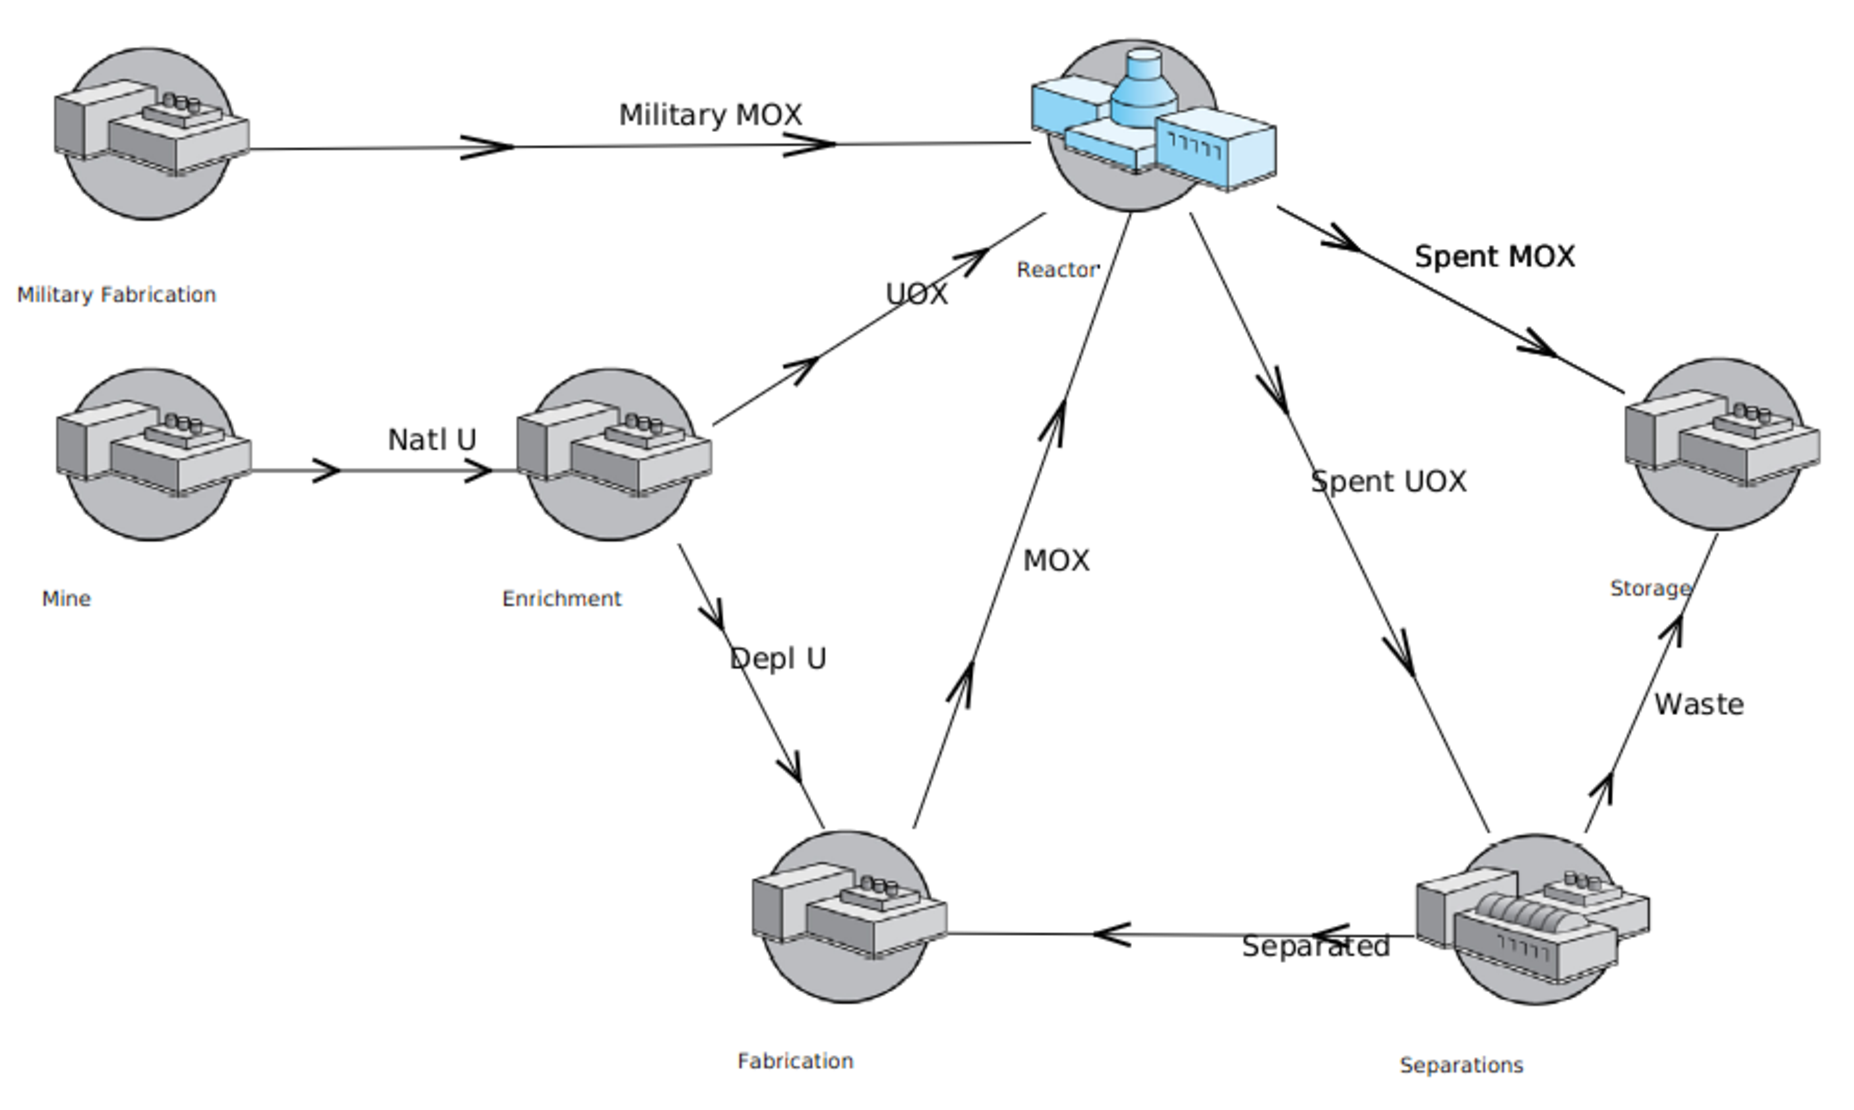
\includegraphics[width=\columnwidth]{military.pdf}
    \caption[]{
      \label{fig:military}
      Material routing between in the \texttt{external} scenario fuel
      cycle. Possible arc flows are labeled with commodity names.}
  \end{center}
\end{figure}

\subsubsection{Regional Tariffs: Fuel Cycles with International Instruments}

One of the novel features of the DRE is the ability for different geographical
and managing entity representations to be laid over otherwise regional-agnostic
fuel cycles and affect the outcome of possible trades between those fuel
cycles. The \texttt{tariff} two-region scenario showcases the ability to model
such situations.

Two regions, Region A and Region B, are modeled. Region A houses a fuel cycle
with both UOX and MOX-based fuels is available. Further, this region has an
over-abundance of supply of fuel and can thus provide fuel services to other
regions. Region B contains a simple, once-through fuel cycle. Both fuel cycles
are shown in Figure \ref{fig:region}.

\begin{figure}
  \begin{center}
    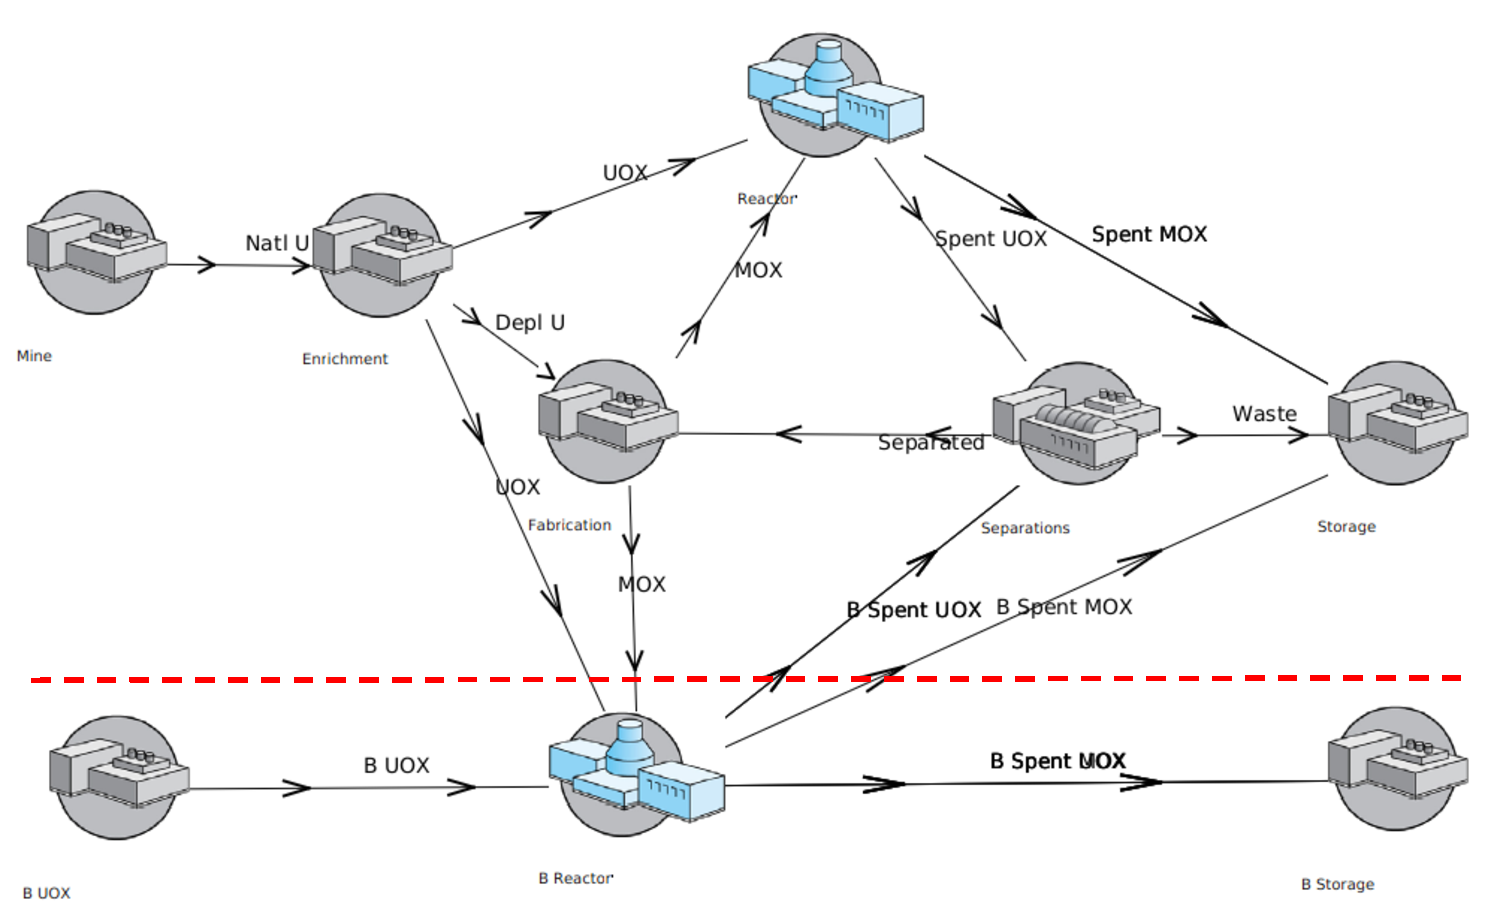
\includegraphics[width=\columnwidth]{region.pdf}
    \caption[]{
      \label{fig:region}
      A two-region set of fuel cycles separated by a dotted-red line. The upper
      region (Region A) includes a one-pass MOX fuel cycle, and the bottom
      region (Region B) includes a once-through fuel cycle connected to the
      one-pass MOX fuel cycle.}
  \end{center}
\end{figure}

Initially, preferences are set such that fuel trade from Region A to
Region B is preferred over Region B's domestic fuel production. In other words, a
preference distribution for fuel supplied to Region B has the following
relation

\begin{equation}\label{eqn:bigdefault}
  p_{MOX, a} > p_{UOX, a} > p_{UOX, b} > 1.
\end{equation}

\noindent
This preference distribution implies that Region B's domestic fuel cycle will
never be utilized -- it will always be fueled by Region A, as long as Region A
has available capacity. 

At some time $t_0$, a time-varying tariff is applied by Region B which perturbs
preference values along arcs connecting Region A fuel suppliers with Region B
fuel consumers. Consider a tariff defined by function in Equation
\ref{eqn:tariff} with preferences adhering to the relation provided in Equation
\ref{eqn:bigp1}, which guarantees a strict preference ordering under $f(t)$.

\begin{equation}\label{eqn:tariff}
f(t)
\begin{cases}
1, & \text{if } t < t_0 \\
\frac{p_{UOX, b} - 1}{p_{UOX, a}}, & \text{if } t_0 \leq t < t_1 \\
\frac{p_{UOX, b} - 1}{p_{MOX, a}}, & \text{if } t_1 \leq t < t_2
\end{cases} 
\end{equation}

\begin{equation}\label{eqn:bigp1}
  p_{UOX, b} \left( 1 - \frac{p_{UOX, a}}{p_{MOX, a}} \right) > 1.
\end{equation}

Choosing nominal values that satisfy Equations \ref{eqn:bigdefault} and
\ref{eqn:bigp1}, e.g., $p_{MOX, a} = 9$, $p_{UOX, a} = 4$, and $p_{UOX, b} = 2$,
one arrives at actual preference values as shown in Figure \ref{fig:prefs}. In
the \texttt{tariff} scenario, $t_0$ is chosen to be 150 and $t_1$ is set to
300. The DRE naturally handles the flow of commodities between Facility agents
in each Region, allowing the application of tariffs by the Region agents.

\begin{figure}
  \begin{center}
    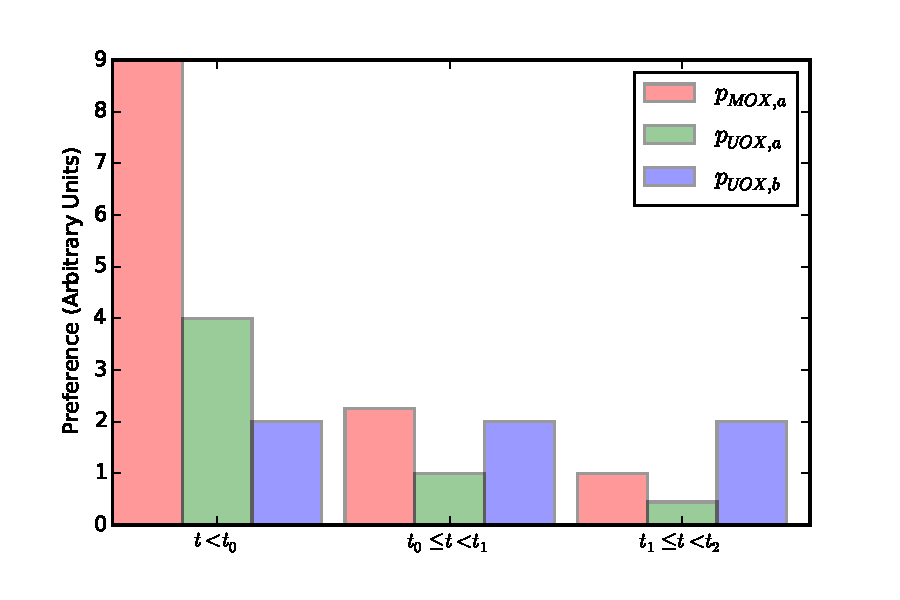
\includegraphics[width=\columnwidth]{tariff_prefs.pdf}
    \caption[]{
      \label{fig:prefs}
      Preference values for reactors in Region B for available fuel commodities
      in Region B as a function of time.}
  \end{center}
\end{figure}

